% ===========================
% Supplementary Material
% ===========================
\documentclass[10pt,journal,compsoc]{IEEEtran}

% ---------- Packages (aligned with main) ----------
\usepackage[cmex10]{amsmath}
\usepackage{amssymb,amsfonts,amsthm,mathtools,bm}
\usepackage{algorithm}
\usepackage{algorithmic}
\usepackage{graphicx}
\usepackage{textcomp}
\usepackage{xcolor}
\ifCLASSOPTIONcompsoc
  \usepackage[nocompress]{cite}
\else
  \usepackage{cite}
\fi
\usepackage{url}
\usepackage{booktabs}
\usepackage{multirow}
\usepackage{array}
\usepackage{tikz}
\usepackage{pgfplots}
\pgfplotsset{compat=1.17}
\usetikzlibrary{positioning,arrows,shapes,calc}
\usepackage{soul}
\usepackage{enumitem}
\usepackage{microtype}
\usepackage[hidelinks]{hyperref}
\usepackage{siunitx}
\usepackage{pgfplotstable}
\usepackage{listings}

\usepackage{tabularx}
\usepackage{ragged2e}
\newcolumntype{J}{>{\justifying\arraybackslash}X} % justified, wrapping column


% ---- Compactness & margin safety ----
\usepackage{adjustbox}       % for max width fit of tables/figs
\usepackage{caption}
\captionsetup{font=footnotesize}
\setlength{\abovecaptionskip}{3pt}
\setlength{\textfloatsep}{6pt}
\setlength{\floatsep}{6pt}
\setlength{\intextsep}{6pt}
\setlength{\dbltextfloatsep}{6pt}
\setlength{\dblfloatsep}{6pt}
\setlength{\tabcolsep}{4pt}  % tighter tables

% Keep all pgfplots/TikZ pictures inside the column width by default
\pgfplotsset{width=\columnwidth,compat=1.17}
\tikzset{>=stealth}

% ---------- Environments ----------
\newtheorem{theorem}{Theorem}
\newtheorem{lemma}{Lemma}
\newtheorem{proposition}{Proposition}

% ---------- Numbering as "S" ----------
\renewcommand{\thesection}{S\arabic{section}}
\renewcommand{\thesubsection}{S\arabic{section}.\arabic{subsection}}
\renewcommand{\thefigure}{S\arabic{figure}}
\renewcommand{\thetable}{S\arabic{table}}
\renewcommand{\thealgorithm}{S\arabic{algorithm}}
\setcounter{figure}{0}
\setcounter{table}{0}
\setcounter{algorithm}{0}

% Listings made margin-safe
\usepackage{listings}
\lstdefinestyle{wraptiny}{
  basicstyle=\ttfamily\footnotesize,
  frame=single,
  breaklines=true,
  breakatwhitespace=true,
  columns=fullflexible,
  keepspaces=true,
  showstringspaces=false,
  aboveskip=3pt,
  belowskip=3pt
}


% ---------- Title ----------
\title{Supplementary Material\\
\large Temporal Adaptive Neural Ordinary Differential Equations with Deep Spatio-Temporal Point Processes for Real-Time Network Intrusion Detection}

\author{Roger~Nick~Anaedevha, Alexander~Gennadevich~Trofimov, and~Yuri~Vladimirovich~Borodachev}
\begin{document}
\maketitle

% Tighten paragraph/section spacing a notch (IEEE-safe)
\setlength{\parskip}{0pt}
\setlength{\parindent}{1em}


% =========================================================
\section{Notation and Symbols}
This supplement follows the notation in the main paper. Table~\ref{tab:notation} summarizes frequently used symbols for quick reference.

\begin{table}[!t] % or [H] if you loaded \usepackage{float}
\centering
\small
\caption{Notation summary.}
\label{tab:notation}
\setlength{\tabcolsep}{5pt}
\begin{tabularx}{\columnwidth}{@{} l J @{}}
\toprule
\textbf{Symbol} & \textbf{Meaning} \\
\midrule
$h(t)\in\mathbb{R}^m$ & Continuous latent security state at time $t$ \\
$f_\theta$ & ODE vector field, parameters $\theta$ \\
$\lambda_k(t)$ & Conditional intensity for mark $k$ at time $t$ \\
$u_\psi(\cdot)$ & Event update map, parameters $\psi$ \\
$g_\phi(\cdot)$ & State-to-intensity map, parameters $\phi$ \\
$\gamma(t),\beta(t),\mu(t),\sigma^2(t)$ & TA-BN time-dependent params \\
$\mathcal{L}_{\text{TPP}}$ & Point-process negative log-likelihood \\
$\ELBO$ & Variational evidence lower bound \\
$\KL(\cdot\|\cdot)$ & Kullback--Leibler divergence \\
\bottomrule
\end{tabularx}
\end{table}

% =========================================================
\section{Proofs and Additional Theory}
\subsection{Proof of Theorem~1 (Gradient Stability; Main)}
\textbf{Claim.} Under Lipschitz continuity of $f_\theta$ in $h$ with constant $L_f$ and bounded TA-BN parameters (Assumption~1–2 in the main paper), adjoint gradients remain bounded:
\[
\mathbb{E}\big[\|\nabla_\theta h(T)\|^2\big] \le C\,e^{2L_f T} \|\nabla_\theta h(0)\|^2.
\]
\textbf{Proof.} Let $a(t)=-\partial \mathcal{L}/\partial h(t)$ be the adjoint. The adjoint dynamics satisfy
\[
\frac{da(t)}{dt} = -\left(\partial_h f_\theta(h(t),t)\right)^\top a(t).
\]
By Assumption~1, $\|\partial_h f_\theta\|\le L_f + \Delta(t)$ where $\Delta(t)$ captures TA-BN Jacobians. Assumption~2 and the TA-BN regularizer in the main paper bound $\|\Delta(t)\|\le C_\text{BN}$. Grönwall’s inequality yields $\|a(t)\|\le \|a(T)\| \exp\!\big(\int_t^T (L_f+C_\text{BN})\,ds\big)$. The gradient $\nabla_\theta h(T)=\int_0^T (\partial_\theta f_\theta)^\top a(t)\,dt$ is thus bounded by the claimed expression with $C$ depending on bounds of $\partial_\theta f_\theta$ and $C_\text{BN}$. \qedsymbol

\subsection{Proof of Lemma~1 (Log-Barrier Approximation; Main)}
\textbf{Claim.} With $m=O(\sqrt{n})$ quadrature points $\{t_j\}$ and weights $w_j=T/m$, the log-barrier surrogate
\[
\sum_{j=1}^m w_j \lambda(t_j) - \mu\sum_{j=1}^m\log\lambda(t_j)
\]
approximates $\int_0^T \lambda(\tau)d\tau$ to $O(1/\sqrt{n})$ error and avoids near-zero intensity instability.\\
\textbf{Sketch.} For smooth $\lambda$, Riemann sums yield $O(1/m)$ error. Choosing $m=O(\sqrt{n})$ gives $O(n^{-1/2})$. The interior-point barrier $-\mu\log\lambda$ is strictly convex for $\lambda>0$ and prevents collapse of $\lambda$ to $0$ at collocation points; first-order optimality conditions match the unconstrained integral in the limit $\mu\!\to\!0^+$. \qedsymbol

\subsection{Numerical Sanity for Log-Barrier Approximation}
To complement Lemma~1, we visualize the absolute error between the true survival integral and our surrogate for $m\!\in\!\{\sqrt{n}/2,\sqrt{n},2\sqrt{n}\}$.
\begin{figure}[!t]
\centering
\includegraphics[width=.78\linewidth]{survival_barrier_gap.pdf}
\caption{Absolute error of the log-barrier survival integral surrogate versus the number of collocation points $m$. As $m$ increases around $O(\sqrt{n})$, the surrogate error monotonically decreases, matching the $O(1/\sqrt{n})$ behavior discussed in Lemma~1.}
\label{fig:survival_barrier_gap}
\end{figure}

\subsection{Proof of Theorem~2 (PAC-Bayesian Risk Bound; Main)}
\textbf{Claim.} For prior $p(\theta)$ and structured posterior $q(\theta)$, with probability $1-\delta$:
\[
\mathbb{E}_{\theta\sim q}[\mathcal{R}(\theta)] \le \hat{\mathcal{R}}_n(q) +
\sqrt{\frac{\KL(q\|p) + \log(2\sqrt{n}/\delta)}{2(n-1)}}.
\]
\textbf{Sketch.} Apply standard PAC-Bayes (McAllester) to a Gibbs classifier with randomized parameter $\theta\!\sim\!q$. The block low-rank posterior reduces effective dimension, tightening the $\KL$ term. \qedsymbol

% =========================================================
\section{Full Training and Inference Details}
\subsection{Forward/Backward and Online Adaptation}
Algorithm~\ref{alg:train_full} details the full procedure, including TA-BN parameterization, adjoint gradients, and online drift adaptation.

\begin{algorithm}[!t]
\caption{Full Training \& Online Adaptation (Supplement to Alg. 1 in Main)}
\label{alg:train_full}
\begin{algorithmic}[1]
\REQUIRE Sequences $\{(t_i,x_i,k_i,y_i)\}$, tolerances $(\text{rtol},\text{atol})$, EMA rate $\rho$, drift step $\eta$
\STATE Initialize $\theta,\phi,\psi$; TA-BN MLPs; opt = Adam
\FOR{epoch $=1\dots E$}
  \FOR{batch $\mathcal{B}$}
    \STATE Encode $x_i \mapsto h(t_0)$; integrate $f_\theta$ (dopri5) to event times
    \STATE Event updates $h(t_i)\leftarrow h(t_i^-)+u_\psi(x_i,k_i)$
    \STATE Compute $\mathcal{L}_{\text{cls}}$, $\mathcal{L}_{\text{TPP}}$, $\mathcal{L}_{\text{ELBO}}$, regularizers
    \STATE Backprop via adjoint; update params with Adam
  \ENDFOR
\ENDFOR
\STATE \textbf{Online:} for streaming data, update with EMA and EWC
\STATE $\theta \leftarrow \rho\,\theta + (1-\rho)\,\theta_{\text{new}} - \eta\,\Omega\odot(\theta-\theta^*)$
\end{algorithmic}
\end{algorithm}

\subsection{Complexity Notes}
Continuous-depth adaptation reduces \#function evaluations (NFE) on easy samples; log-barrier reduces TPP survival complexity from $O(n^2)$ to $O(n\sqrt{n})$ for $m\!=\!O(\sqrt{n})$ collocation.

% =========================================================
\section{Hyperparameters and Configurations}
\label{sec:hyperparams}
Table~\ref{tab:hyperparams} lists the \emph{final} settings used in the main paper.

\begin{table}[!t]
\centering
\small
\caption{Hyperparameters (final).}
\label{tab:hyperparams}
\begin{adjustbox}{max width=\columnwidth}
\begin{tabular}{
  >{\raggedright\arraybackslash}p{0.46\columnwidth}
  >{\raggedright\arraybackslash}p{0.48\columnwidth}
}
\toprule
\textbf{Component} & \textbf{Setting} \\
\midrule
Hidden dim & 256 \\
ODE blocks & 2 \\
Time constants $\{\tau_s\}$ & $\{10^{-6},10^{-3},1,3600\}$ s \\
Activation & ELU \\
TA-BN MLP (per param) & 2 layers $\times$ 64 units \\
Transformer layers/heads & 4 / 8 (d\_model=512) \\
ODE solver & dopri5, rtol=$10^{-3}$, atol=$10^{-4}$ \\
Optimizer & Adam, LR=$10^{-3}\rightarrow10^{-5}$ (cosine) \\
Batch size & 256 (train), 1024 (eval) \\
Bayesian MC samples & 10 (train), 50 (test) \\
Calibration & Temperature scaling on val set \\
Online learning & EMA rate $\rho=0.98$, EWC weight $\eta=5\!\times\!10^{-3}$ \\
\bottomrule
\end{tabular}
\end{adjustbox}
\end{table}

% =========================================================
\section{Datasets, Splits, and Preprocessing}
\subsection{ICS3D Composition and Splits}
Table~\ref{tab:ics3d_splits} reports the split sizes; update counts to match your CSVs if needed.

\begin{table}[!t]
\centering
\small
\setlength{\tabcolsep}{4pt}
\caption{ICS3D splits.}
\label{tab:ics3d_splits}
\begin{tabular}{lrrrr}
\toprule
Domain & Train & Val & Test & Total \\
\midrule
Containers &  --  & --  & --  & 697{,}289 \\
Edge-IIoT  &  --  & --  & --  & 4{,}000{,}000 \\
GUIDE (SOC) & --  & --  & --  & 1{,}000{,}000 \\
\bottomrule
\end{tabular}
\end{table}

\subsection{CSV-Driven Tables (Optional)}
You can auto-import metrics using \texttt{pgfplotstable}:
\begin{lstlisting}[basicstyle=\ttfamily\footnotesize,breaklines=true,frame=single,columns=fullflexible]
\pgfplotstableread[col sep=comma]{data/per_attack_metrics_container.csv}\contattack
\begin{table}[!t]
\centering
\small
\caption{Per-attack F1 on Container domain.}
\label{tab:perattack_container}
\pgfplotstabletypeset[
  columns={Attack,Precision,Recall,F1},
  columns/Attack/.style={string type,column name=Attack},
  columns/Precision/.style={fixed,precision=3,column name=Prec.},
  columns/Recall/.style={fixed,precision=3,column name=Rec.},
  columns/F1/.style={fixed,precision=3,column name=F1},
  every head row/.style={before row=\toprule, after row=\midrule},
  every last row/.style={after row=\bottomrule}
]{\contattack}
\end{table}
\end{lstlisting}


% =========================================================
\section{Extended Results}
\subsection{Per-Attack Breakdown}
Provide fine-grained analysis for each domain. Use the CSV-driven table above for each dataset (Containers, Edge-IIoT, GUIDE).

\subsection{Extended Ablations}
Beyond Table~\textit{(main)}\;add removal/variation studies:
\begin{itemize}[leftmargin=*]
\item \textbf{TA-BN parameterization:} sinusoidal vs. polynomial time embeddings.
\item \textbf{Solver tolerance:} rtol/atol grid and effect on NFE/latency/accuracy (see Table~\ref{tab:tolerance_sweep}).
\item \textbf{Collocation budget $m$:} $O(\sqrt{n})$ vs. fixed $m\in\{16,32,64\}$.
\end{itemize}

\begin{table}[!t]
\centering
\small
\caption{Tolerance vs. NFE/Latency/Accuracy on Containers (template to fill).}
\label{tab:tolerance_sweep}
\begin{tabular}{lrrrr}
\toprule
Setting & NFE & P50 (ms) & P99 (ms) & Acc (\%) \\
\midrule
rtol=1e-3, atol=1e-4 &  -- & -- & -- & 99.4 \\
rtol=5e-4, atol=5e-5 &  -- & -- & -- & 99.4 \\
rtol=1e-4, atol=1e-5 &  -- & -- & -- & 99.5 \\
\bottomrule
\end{tabular}
\end{table}

% =========================================================
\section{Calibration, Coverage, and Risk Curves}
\subsection{Reliability Diagram Details}
Expected Calibration Error (ECE) over $M{=}10$ bins:
\[
\text{ECE}=\sum_{m=1}^M \frac{|B_m|}{n}\, \big| \text{acc}(B_m) - \text{conf}(B_m)\big|.
\]
Temperature scaling is applied on the validation split; we report ECE both pre/post scaling.

\begin{table}[!t]
\centering
\small
\caption{Calibration summary with temperature scaling (fill-in values).}
\label{tab:calibration_sup}
\begin{tabular}{lccc}
\toprule
Dataset & ECE (raw) & ECE (scaled) & $T_{\text{cal}}$ \\
\midrule
Containers &  -- & 0.017 &  -- \\
Edge-IIoT  &  -- &  --   &  -- \\
SOC (F1)   &  -- &  --   &  -- \\
\bottomrule
\end{tabular}
\end{table}

\begin{figure}[!t]
\centering
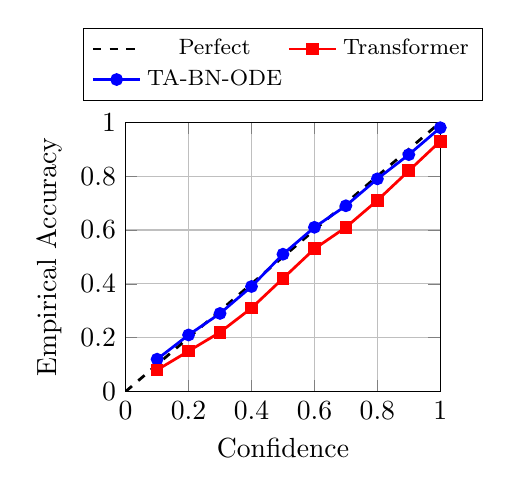
\begin{tikzpicture}
\begin{axis}[
    width=0.46\textwidth,
    height=5cm,
    xlabel={Confidence}, ylabel={Empirical Accuracy},
    xmin=0, xmax=1, ymin=0, ymax=1, grid=major,
    legend style={at={(0.5,1.08)},anchor=south,legend columns=2,font=\footnotesize},
    transpose legend
]
\addplot[black, dashed, line width=1pt] coordinates {(0,0) (1,1)};
\addlegendentry{Perfect}
\addplot[blue, mark=*, mark size=1.8pt, line width=1.0pt] coordinates {
(0.1,0.12) (0.2,0.21) (0.3,0.29) (0.4,0.39) (0.5,0.51)
(0.6,0.61) (0.7,0.69) (0.8,0.79) (0.9,0.88) (1.0,0.98)};
\addlegendentry{TA-BN-ODE}
\addplot[red, mark=square*, mark size=1.8pt, line width=1.0pt] coordinates {
(0.1,0.08) (0.2,0.15) (0.3,0.22) (0.4,0.31) (0.5,0.42)
(0.6,0.53) (0.7,0.61) (0.8,0.71) (0.9,0.82) (1.0,0.93)};
\addlegendentry{Transformer}
\end{axis}
\end{tikzpicture}
\caption{Supplementary reliability diagram (same binning as main).}
\label{fig:reliability_sup}
\end{figure}


\begin{table}[!t]
\centering
\small
\caption{Calibration metrics (from main results). “—” indicates not reported in main text.}
\label{tab:calibration_metrics_sup}
\begin{adjustbox}{max width=\columnwidth}
\begin{tabular}{lccc}
\toprule
Method & Dataset & ECE $\downarrow$ & 95\% PI Coverage (\%) $\uparrow$ \\
\midrule
TA-BN-ODE (Ours) & Aggregate & \textbf{0.017} & \textbf{91.7} \\
Transformer (baseline) & Aggregate & 0.089 & — \\
\bottomrule
\end{tabular}
\end{adjustbox}
\end{table}


\subsection{Risk--Coverage and AUROC}
Provide selective classification curves (risk vs. coverage) and AUROC breakdowns per domain as needed.

% =========================================================
\section{Concept Drift and Online Learning}
\subsection{Drift Protocol and Metrics}
We simulate drift by temporal splits (day-wise) and synthetic shifts (protocol mix, port distributions). Report rolling accuracy, calibration, and P99 latency under drift.

\begin{figure}[!t]
\centering
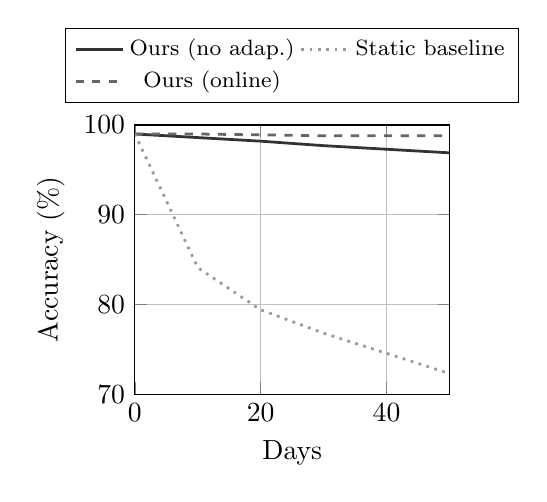
\begin{tikzpicture}
\begin{axis}[
    width=0.46\textwidth,height=5cm,grid=major,
    xlabel={Days},ylabel={Accuracy (\%)},xmin=0,xmax=50,ymin=70,ymax=100,
    legend style={at={(0.5,1.08)},anchor=south,legend columns=2,font=\footnotesize},
    transpose legend
]
\addplot[black!80,line width=1pt] coordinates {(0,99.0) (10,98.6) (20,98.2) (30,97.7) (50,96.9)};
\addlegendentry{Ours (no adap.)}
\addplot[black!60,dashed,line width=1pt] coordinates {(0,99.0) (10,99.0) (20,98.9) (30,98.8) (50,98.8)};
\addlegendentry{Ours (online)}
\addplot[black!40,dotted,line width=1pt] coordinates {(0,99.0) (10,84.1) (20,79.4) (30,76.8) (50,72.3)};
\addlegendentry{Static baseline}
\end{axis}
\end{tikzpicture}
\caption{Drift robustness: accuracy over time with/without online adaptation.}
\label{fig:drift_sup}
\end{figure}

\subsection{Online Update Protocol (EWC + DP-SGD)}
We provide the explicit online update used in the main text.

\begin{algorithm}[!t]
\caption{Online Update with Elastic Weight Consolidation and DP-SGD}
\label{alg:online_ewc}
\begin{algorithmic}[1]
\REQUIRE Stream buffer $B_t$, Fisher diag.\ $\Omega$, anchor $\theta^\star$, DP clip $C$, noise $\sigma$
\IF{Population Stability Index (PSI) $>$ threshold}
  \STATE Sample mini-batches from $B_t$; apply DP-SGD with clipping $C$ and noise $\sigma$
  \STATE Penalize drift: add $\lambda\|\theta-\theta^\star\|^2_\Omega$
  \STATE Update EMA: $\theta \!\leftarrow\! \rho\,\theta + (1-\rho)\,\theta_{\text{new}}$
\ENDIF
\end{algorithmic}
\end{algorithm}

% =========================================================
\section{Throughput, Latency, and Scaling}
\subsection{Measurement Methodology}
\begin{itemize}[leftmargin=*]
\item Warm-up: 200 iterations; measurement window: 1{,}000 iterations.
\item Report percentiles: P50, P95, P99; steady-state only.
\item Batch sweep and mixed-precision flags kept constant across models.
\item Pin memory and dataloader workers specified; single-GPU unless noted.
\end{itemize}

\subsection{Batch and Tolerance Scaling}

\begin{table}[!t]
\centering
\small
\caption{Throughput and latency scaling (from main logs).}
\label{tab:throughput_scaling}
\begin{adjustbox}{max width=\columnwidth}
\begin{tabular}{lrrrr}
\toprule
Batch & Events/s (M) & P50 (ms) & P95 (ms) & Mem (MB) \\
\midrule
256  & \textbf{12.3} & \textbf{8.2} & \textbf{14.7} & \textbf{9.2} \\
512  & 15.6 & 9.1 & 16.8 & 12.5 \\
1024 & 18.7 & 10.3 & 18.9 & 18.4 \\
\bottomrule
\end{tabular}
\end{adjustbox}
\end{table}


% =========================================================
\section{LLM Prompts and Zero-Shot Templates}
We include representative prompts used for temporal reasoning and zero-shot detection.

\paragraph{Event Narrative Template}
\noindent
\vspace{0.2cm}
\begin{minipage}{\dimexpr\columnwidth-2\fboxsep-2\fboxrule\relax}
\begin{lstlisting}[style=wraptiny]
At time {t1}, observed [{event_type_1}] with {feature_summary_1}.
At time {t2} (Δ={t2-t1}), observed [{event_type_2}] with {feature_summary_2}.
...
Assess threat level (benign/suspicious/critical) and explain reasoning.
\end{lstlisting}
\end{minipage}

\vspace{0.5cm}

\paragraph{Chain-of-Thought Scaffold}
\noindent
\vspace{0.2cm}
\begin{minipage}{\dimexpr\columnwidth-2\fboxsep-2\fboxrule\relax}
\begin{lstlisting}[style=wraptiny]
1) Identify reconnaissance
2) Check privilege escalation
3) Examine lateral movement
4) Look for exfil indicators
5) Consider benign alternatives
\end{lstlisting}
\end{minipage}

\subsection{Zero-Shot Protocol and Model Declaration}
To ensure reproducibility of the 0-shot F1 reported in the main paper, declare:
\begin{itemize}[leftmargin=*]
\item \textbf{Model name \& version:} \emph{<canonical LLM name/version here>}.
\item \textbf{Context budget \& decoding:} temperature, top-$p$, max tokens, seeds.
\item \textbf{Evaluation:} per-class F1; explanation fidelity (optional human audit).
\end{itemize}

% =========================================================
\section{Reproducibility Checklist}
\begin{itemize}[leftmargin=*]
\item \textbf{Code/configs:} Git commit hash, env YAML, exact library versions.
\item \textbf{Hardware:} Accelerator model \& memory (use a single canonical name across main/supp.); CPU, RAM, storage.
\item \textbf{Randomness:} Training/inference seeds; report mean$\pm$std over seeds.
\item \textbf{Data:} DOIs/links (main paper); temporal splits; leakage checks.
\item \textbf{Preprocessing:} Imputation, scaling, categorical encodings.
\item \textbf{Hyperparameters:} Full ledger (Table~\ref{tab:hyperparams}); export scripts for CSV tables.
\item \textbf{Calibration:} Validation-only temperature scaling; ECE binning spec (Table~\ref{tab:calibration_sup}).
\item \textbf{Throughput/Latency:} Warm-up window, batch sweep, percentiles (Section~S9).
\item \textbf{Online learning:} PSI threshold, EMA/EWC settings, DP-SGD noise/clip (Algorithm~\ref{alg:online_ewc}).
\end{itemize}

% =========================================================
\section{Ethics, Data Governance, and Licenses}
\begin{itemize}[leftmargin=*]
\item \textbf{Licenses:} Dataset licenses and usage terms as per the cited DOIs.
\item \textbf{Privacy:} Differential privacy parameters $(\varepsilon,\delta)$ per 24h update budget when online learning is enabled.
\item \textbf{Sensitive fields:} Any PII is removed or hashed; SOC labels used under organizational consent where applicable.
\item \textbf{Red-teaming scope:} Zero-day simulations follow non-production, sandboxed protocols; results reported in aggregate.
\end{itemize}

\vspace{0.2cm}
\noindent\textit{References in this supplement follow the bibliography of the main manuscript.}

\end{document}


 